
\chapter{Loops}
\label{ch:loops}

\index{non-linear}
\index{loop}

It's time for our first look at a \textbf{non-linear} program. Up to now, all
of our Python programs have executed step-by-step, start to finish, like a
metronome, with each line of code getting executed exactly once. That's about
to change. In this chapter, we introduce the concept of a \textbf{loop}, which
is a programming construct that directs lines of code to be executed
\textit{repeatedly}, and out of strict sequence.

\section{The two species of loops}

\index{fixed-iteration (loop)}
\index{variable-iteration (loop)}
\index{counter-controlled (loop)}
\index{condition-controlled (loop)}
\index{for loop@\texttt{for} loop}
\index{while loop@\texttt{while} loop}

Although some programming languages try to dress them up further, there are
really only two fundamental kinds of loops in the world:
\textbf{fixed-iteration loops} and \textbf{variable-iteration
loops}.\footnote{Sometimes these are called \textbf{counter-controlled} and
\textbf{condition-controlled} loops, respectively.} The first kind is simpler
to understand and less error-prone; in most languages (Python included) it is
implemented as a ``\textbf{\texttt{for} loop}.'' The tricker, second kind is
available to programmers as a ``\textbf{\texttt{while} loop}.''

Happily for us, it turns out that \texttt{while} loops don't come up much in
Data Science, at least in the beginning. There are some more advanced
techniques that use them (for instance, optimization methods and threshold
detection) but for us it's going to be \texttt{for} loops that dominate the
landscape. So let's figure out how they work.

\section{A word of caution}

\index{query}

But before we embark, a cautionary note. Some of the things that loops can do
-- especially the early examples -- can also be done using the queries of the
last chapter. For instance, we could use a query to find all the strings in a
\texttt{Series} that begin with the letter \texttt{T}, or we could use a loop
to do the same thing.

Here's the rule: \textbf{if you can do it without a loop, that is always
preferred.} There are two reasons for this. First, it's less code to write, and
less error-prone, to use Pandas' built-in features rather than crafting a loop
yourself. That's why they created those features (like queries) after all.

Second, and ultimately even more important, using a Pandas function is
\textit{much faster} to execute than a loop. The reason has to do with how a
loop is eventually broken down into the little instructions a machine can
understand: when Python runs a loop, it plods through the steps methodically,
whereas the Pandas functions are all pre-baked into a water-cooled rocket
engine that can jet out of the gate.

You don't need to know any of those nitty-gritty details. All you have to
remember is: don't ever resort to using a loop unless you can't figure out how
to do what you want without one. (And unfortunately, there are indeed those
times.)

\section{Iterating through an array}

\label{arrayLoops}
\index{iterate}

Most often, we'll use a \texttt{for} loop to ``loop through,'' or
``\textbf{iterate} through,'' the contents of an aggregate data variable. This
means that instead of executing a snippet of code \textit{once}, we'll execute
it \textit{once per element of the variable}. This ``once per element'' thing
is what makes the code non-linear.

\index{array}
\index{ndarray@\texttt{ndarray} (NumPy)}

Let's start with the first aggregate data type we learned, a NumPy array.

\begin{Verbatim}[fontsize=\small,samepage=true,frame=single,framesep=3mm]
 1: villains = np.array(['Jafar','Ursula','Maleficent','Gaston'])
 2: print("Here we go!")
 3: for villain in villains:
 4:     print("Oooo, {} is scary!".format(villain))
 5:     print("({} has {} letters.)".format(villain, len(villain)))
 6: print("Whew!")
\end{Verbatim}

\index{loop!header}
\index{loop!body}

(I've numbered the lines in this example so I can refer to them in the text
below, but the numbers and colons aren't part of Python.)

Immediately after creating our \texttt{villains} array, and printing an
introductory message, we encounter our first loop. A loop consists of two
parts: the \textbf{loop header} and the \textbf{loop body}. Here are the rules:

\index{indentation}
\index{curlies (curly braces)}
\index{\{\}@\texttt{\{\}} (curlies)}

\begin{compactitem}
\item The loop header consists of the line that begins with ``\texttt{for}''.
\item The loop body consists of \textit{all of the consecutive following lines
that are \textbf{indented} (tabbed-over) one tab.}\footnote{Other programming
languages -- every other one I know besides Python, in fact -- uses some other
way to designate the loop body than indentation. Many (R and Java, for
instance) use curly braces before and after the loop body so that the computer
knows where it begins and ends. I personally like this feature of Python's, but
there are haters, and the bottom line is you just have to get used to it.}
\end{compactitem}

That second rule turns out to be more important than it seems at first. A very
(\textit{very!}) common error among beginners is to ``mis-indent'' their code
such that their loop body includes more, or less, than they mean it to. So
heads up.

Before we continue, stare at that code above and convince yourself of these two
facts:

\begin{compactitem}
\item[\leftpointright] The loop header is line \textbf{3}.
\item[\leftpointright] The loop body is lines \textbf{4 and 5}. (\textit{Not} line 4
only! \textit{Not} lines 4, 5, and 6!)
\end{compactitem}

\medskip
Now the reason this is important is that a \texttt{for} loop works as follows:
\vspace{-.1in}

\index{memory picture}

\definecolor{shadecolor}{rgb}{.9,.9,.9}
\begin{shaded}
\begin{compactenum}
\itemsep.1em
\item First, create a new variable (on the left-hand side of the memory
picture) named whatever comes immediately after the word ``\texttt{for}''. (In
this example, the name of this new variable will be \texttt{villain}.)
\item Then, for \textit{each} element of the array, in succession:
    \begin{compactenum}
    \itemsep.1em
    \item Set that variable's value to the next element of the array.
    \item \textit{Execute the entire loop body.} (In this example, lines 4--5.)
    \end{compactenum}
\end{compactenum}
\end{shaded}

In the \texttt{villains} example, therefore, the lines in order of execution
are:

\begin{center}
1, 2, 3, 4, 5, 3, 4, 5, 3, 4, 5, 3, 4, 5, 6.
\end{center}

(Do you agree?)

The memory picture changes constantly throughout any program, including those
that contain loops. Let's take a snapshot of memory as it appears immediately
after executing line 3 the \textit{second} time. In other words, we'll run the
program this far before hitting the pause button:

\begin{center}
1, 2, 3, 4, 5, 3, \textit{Freeze!!}
\end{center}

\index{loop variable}

Memory at this instant is depicted in Figure~\ref{fig:loopsMemory}. The second
time we executed line 3, we set \texttt{villain} (sometimes called the
\textbf{loop variable}, by the way) to the second element of the array,
\texttt{"Ursula"}. We're just about to execute line 4 for the second time. Note
that the \texttt{villains} array is unaffected by this entire loop process:
only our temporary, made-up loop variable (\texttt{villain}) gets a new value
each time.

\begin{figure}[ht]
\centering
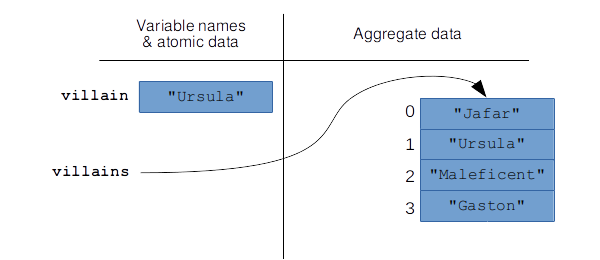
\includegraphics[width=0.8\textwidth]{loopsMemory.png}
\caption{A snapshot of memory immediately after the \textit{second} execution
of line \textit{3} of the \texttt{villains} program.}
\label{fig:loopsMemory}
\end{figure}

The complete output of the program, as you can easily deduce, is thus:

\begin{Verbatim}[fontsize=\small,samepage=true,frame=leftline,framesep=5mm,framerule=1mm]
Here we go!
Oooo, Jafar is scary!
(Jafar has 5 letters.)
Oooo, Ursula is scary!
(Ursula has 6 letters.)
Oooo, Maleficent is scary!
(Maleficent has 10 letters.)
Oooo, Gaston is scary!
(Gaston has 6 letters.)
Whew!
\end{Verbatim}

Don't miss the fact that the ``\texttt{scary!}''~and ``\texttt{has $n$
letters}'' messages were printed four times each, whereas
``\texttt{Whew!}''~only appeared once. That has everything to do with the
indentation: it told Python that lines 4 and 5 \textit{were} part of the loop
body, whereas line 6 was just ``business as usual,'' taking place only after
all the loop hoopla was over and done with.

\section{Iterating through the values of a \texttt{Series}}

\label{seriesLoops}
\index{iteration}

Great news: if you mastered the previous section, this one and the next will be
a snap. That's because Python, NumPy, and Pandas work together to make
iterating through a \texttt{Series} pretty much \textit{exactly the same} as
iterating through an array. In fact, sometimes you're not even sure which type
you've got!

\index{Marvel comics}

Here's the Marvel \texttt{Series} regurgitated yet again:

\begin{Verbatim}[fontsize=\small,samepage=true,frame=single,framesep=3mm]
alter_egos = pd.Series(['Hulk','Spidey','Iron Man','Thor'],
    index=['Bruce','Peter','Tony','Thor'])
\end{Verbatim}

\index{Thanos}
\index{snap@``the snap''}

Let's say I want to go through and greet all our heroes. It's a snap! (no pun
intended):

\begin{Verbatim}[fontsize=\small,samepage=true,frame=single,framesep=3mm]
print("Welcome to the Marvel Cinematic Universe(tm).")
for hero in alter_egos:
    print("Greetings, {}!".format(hero))
print("Go team!")
\end{Verbatim}

\begin{Verbatim}[fontsize=\small,samepage=true,frame=leftline,framesep=5mm,framerule=1mm]
Welcome to the Marvel Cinematic Universe(tm).
Greetings, Hulk!
Greetings, Spidey!
Greetings, Iron Man!
Greetings, Thor!
Go team!
\end{Verbatim}

What could be easier?

Notice that ``looping through the \texttt{Series}'' effectively means ``looping
through the \textit{values} of the \texttt{Series},'' not the keys. What if we
want to loop through the keys instead?

\section{Iterating through the keys of a \texttt{Series}}

\index{iteration}
\index{index@\texttt{.index} syntax (Pandas)}

I'm glad you asked. But in fact, you already know the answer: just use the
\texttt{.index} syntax from p.~\pageref{dotIndex}!

\begin{Verbatim}[fontsize=\small,samepage=true,frame=single,framesep=3mm]
print("Let's iterate through the keys instead:")
for secret_identity in alter_egos.index:
    print("Nice to meet you, {}.".format(secret_identity))
print("Carry on...")
\end{Verbatim}

\begin{Verbatim}[fontsize=\small,samepage=true,frame=leftline,framesep=5mm,framerule=1mm]
Let's iterate through the keys instead:
Nice to meet you, Bruce.
Nice to meet you, Peter.
Nice to meet you, Tony.
Nice to meet you, Thor.
Carry on...
\end{Verbatim}

\index{loop variable}

By the way, you can see that the name of the loop variable is completely at
your discretion. I called the previous one ``\texttt{hero}'' and this one
``\texttt{secret\_identity}'' just because those names were reflective of their
contents. But it's really up to you: it has nothing to do with the name of the
\texttt{Series} itself. (Yeah, I know the Marvel identities aren't secret
anymore, but I'm old school.)

\section{Iterating through the keys \textit{and} values of a \texttt{Series}}

\index{items@\texttt{.items()} (Pandas)}

Finally, it's common to need access to both halves of each key/value pair as
you iterate through a \texttt{Series}. The way to accomplish this is to call
the \texttt{.items()} method of the \texttt{Series}. But it's tricky, because
when you use \texttt{.items()} you assign \textit{two} variables in your loop
instead of just one.

Before showing the complete loop, let's focus on just the loop header needed
for this technique:

\begin{Verbatim}[fontsize=\normalsize,samepage=true,frame=single,framesep=3mm]
for secret_identity, hero in alter_egos.items():
\end{Verbatim}

I named two loop variables, separated by a comma. The reason I put
\texttt{secret\_identity} first is that in this \texttt{Series}, we used
\texttt{Bruce}, \texttt{Peter}, \textit{etc.} as the \textit{keys}, with the
superhero names as the values. And with \texttt{.items()}, the variable name
you want to use for the key is listed first.

The rest of the loop follows logically from this, with both variables available
inside the loop body:

\begin{Verbatim}[fontsize=\small,samepage=true,frame=single,framesep=3mm]
print("We're now going to recognize some outstanding citizens.")
for secret_identity, hero in alter_egos.items():
    print("{}, known to his friends as {}.".format(hero, secret_identity))
    print("The crowd screams: 'YAY {}!'".format(hero.upper()))
print("Thanks, everyone, for your service.")
\end{Verbatim}

If we freeze the program just after the \textit{third} execution of the loop
header this time, we get the picture in Figure~\ref{fig:loopsMemory2}. And the
output, of course, is:

\begin{Verbatim}[fontsize=\small,samepage=true,frame=leftline,framesep=5mm,framerule=1mm]
We're now going to recognize some outstanding citizens.
Hulk, known to his friends as Bruce.
The crowd screams: 'YAY HULK!'
Spidey, known to his friends as Peter.
The crowd screams: 'YAY SPIDEY!'
Iron Man, known to his friends as Tony.
The crowd screams: 'YAY IRON MAN!'
Thor, known to his friends as Thor.
The crowd screams: 'YAY THOR!'
Thanks, everyone, for your service.
\end{Verbatim}

\begin{figure}[ht]
\centering
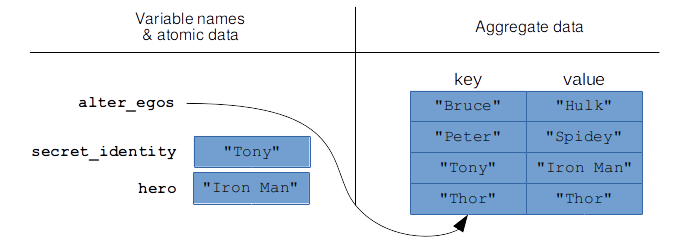
\includegraphics[width=0.9\textwidth]{loopsMemory2.png}
\caption{A snapshot of memory immediately after the \textit{third} execution
of the loop header in the \texttt{alter\_egos} program.}
\label{fig:loopsMemory2}
\end{figure}

\section{Wrapping up}

We can, of course, do much more inside loops than just print things. We can
perform computations galore. The examples in this chapter were simply to
illustrate the structure and behavior of \texttt{for} loops, so that you have a
framework for understanding how more complex parts fit into them later.

Onward!
